\subsection{Overview}
The following text outlines the comprehensive methodology adopted to conduct a comparative analysis of mobile application development approaches using Java, Kotlin, and Dart. The primary objective of this research is to evaluate and compare the development efficiency, code maintainability, and overall quality of applications developed across these three different programming languages. The methodology is divided into two distinct but interrelated parts to achieve a robust analysis.
\par
\textbf{Part I: Identical Mobile Application Development}—This segment focuses on the practical aspect of developing an identical Kanban board application across the three selected programming languages. It involves setting up development environments, detailing the application features and implementation strategies, and standardizing development processes to ensure comparability. This part aims to directly assess the hands-on development experiences and the intrinsic differences in coding practices, development time, and initial code quality among Java, Kotlin, and Flutter.
\par
\textbf{Part II: SonarQube Code Inspection and Open Source Projects} - The second part of the methodology utilizes SonarQube, a tool for measuring code quality, to conduct an extensive analysis of existing open-source projects written in Java, Kotlin, and Dart. This includes a detailed setup of the SonarQube environment, a selection of projects based on predefined criteria, and systematic code inspections. The goal is to objectively evaluate and compare code quality in terms of maintainability, prevalence of code smells, and other quality metrics across projects that use these technologies.
\par
The dual perspective on software development practices provided by both parts, direct through application development and indirect through analysis of existing codebases, enriches the understanding of each languages's capabilities and limitations and enhances the reliability of the study by cross-verifying findings from practical development with empirical data from broader project analyses.
\par
By combining these methodologies, the research aims to deliver insightful conclusions that can guide developers in selecting the most suitable programming language based on empirical evidence and practical experiences. The subsequent sections will detail each part of the methodology, explaining the processes, tools, and criteria used to ensure a thorough and unbiased evaluation of each development approach.
\subsection{Identical Mobile Application Development}
The present study outlines a methodology for investigating the efficacy of three programming languages, Java, Kotlin, and Dart, by developing an identical Kanban board application. The investigation aims to evaluate each language's development efficiency, usability, and initial code quality. The study provides a comprehensive account of the developmental process followed for each language, ensuring that the functional parity of the application is maintained while adhering to the conversational practices of each programming language.
\subsubsection{Project Planning.}
The initial phase of our research project involved identifying an appropriate application to develop to assess which language would be best suited for project development and maintenance. The application needed advanced features to achieve this objective while remaining relatively uncomplicated. Initially, an e-commerce application was proposed. However, after careful consideration, it was determined that the backend development required for such an application would be too time-consuming. Consequently, a To-do application was chosen to fulfill the research objectives of identifying a language best suited for application development.
\par

In the next phase of project development, the features to include and the backend and database to use were meticulously evaluated. After thorough consideration, it was concluded that Firebase is the optimal choice for the backend. This decision was primarily driven by Firebase’s significantly reduced coding effort, thanks to its extensive range of pre-built features that seamlessly integrate into the project. Moreover, Firebase offers two database options—Realtime and Firestore—and Firestore was selected for its superior performance and scalability.
\par
Once the database was settled on, a user-centric approach to feature selection was embarked upon. The features that best serve the project’s needs were identified. The following features were chosen:
\begin{itemize}
\item	Kanban Board Visualization: A visually appealing layout representing tasks across stages—to-do, In Progress, and Completed.
\item	User Account Management includes user registration, login/logout, and the option to log in with Google.  
\item  	Task Management is adding new tasks, editing and modifying existing tasks, and moving tasks between different stages.
\item 	Time Tracking: This stopwatch feature allows users to track the time spent on tasks in the \verb|"In Progress"| stage and pause the timer by moving tasks back to the To-Do stage.
\item 	Export and Share Functionality: Users can export their tasks as a CSV file and share them with others.
\item   Database Integration: The Firebase database is utilized to store and manage user data and tasks, enabling real-time updates and synchronization across all devices.
\end{itemize}

\begin{figure}[htbp]
    \centering
    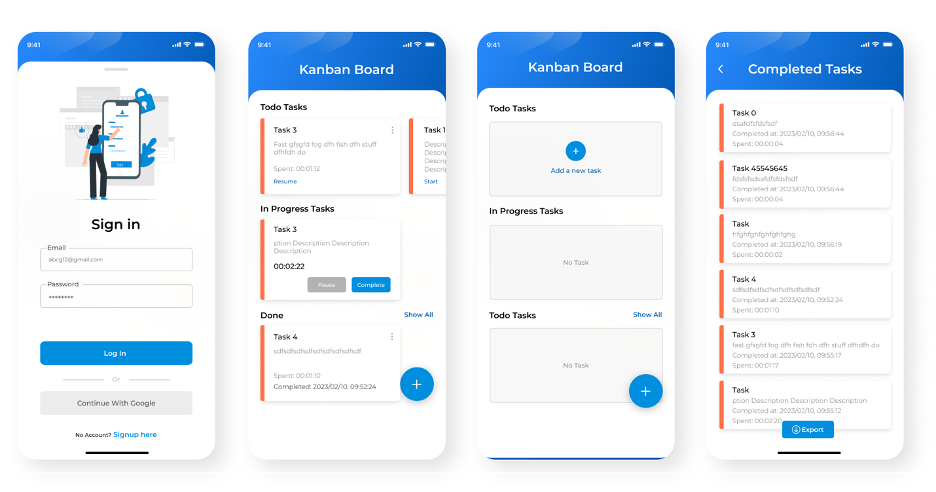
\includegraphics[scale = 0.85]{img/kanban_board.png}
    \caption{Planned view of Kanban Board Application. Designed Using Figma}
    \label{fig:kanban_board}
\end{figure}

\par
The next step was to create a detailed design for the application. After some consideration, the Figma application was chosen due to its widespread popularity in app and web development. Establishing a comprehensive feature plan and precise design before commencing the coding process is essential. With a clear objective in mind, the importance of avoiding improvisation was recognized, leading to the decision to prioritize the design phase before diving into coding.
\par
Following the design phase of the project, during which Figma was utilized to create a comprehensive plan for the application, critical decisions regarding feature selection and the choice of database and backend service were made. With these decisions finalized, the project was poised to embark on the development phase, beginning with the coding part.
\begin{figure}[htbp]
    \centering
    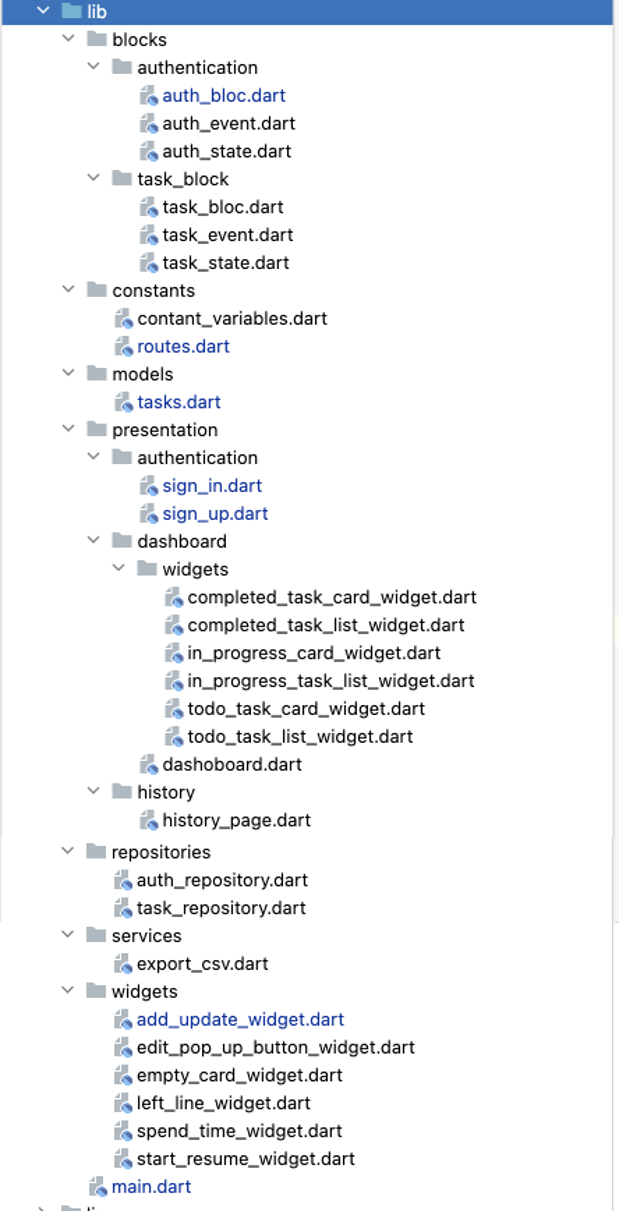
\includegraphics[scale = 0.8]{img/flutter_app_str.png}
    \caption{Flutter version of the application’s project structuring}
    \label{fig:flutter_app_str}
\end{figure}
\subsubsection{Flutter Application Development}
The Flutter application was chosen as the starting point to ensure a smooth development process due to familiarity with the language. With feature specifications and Figma designs already in place, the process was streamlined. BLOC \cite{bloc} was chosen for state management, which is highly regarded in the Flutter community for its reliability and ease of maintenance. Although it may require some practice and digging to get started, compared to other state management approaches like GetX \cite{getX} and Provider \cite{provider}, BLOC is known for its reliability and ease of maintaining advantages. It is used solely for the business logic of the application and state management, separating it from the presentation layer. The three main components of BLOC are Events, States, and Blocs. User interactions trigger Events sent to a Bloc, which processes them and performs any necessary logic, such as data fetching or computations. The Bloc then emits a new State based on the results, and the UI listens to these state changes to update itself accordingly. This architecture enhances maintainability and testability by decoupling the UI from the core business logic.

\par
The project took approximately 20 hours to complete, resulting in a total of 29 files. As the Figure \ref*{fig:flutter_app_str} shows, the project was divided into directories. The project is organized into several directories: blocks contain BLoC components for authentication and task management, managing logic, events, and states; constants directory includes global constants and routing configurations; models define the task data model; presentation houses UI screens for authentication, a dashboard with various widgets for displaying tasks based on their status, and a history page for viewing completed tasks or activity logs; repositories manage data operations related to authentication and tasks, interfacing with databases or APIs; services includes functionalities such as exporting task data to CSV files; and widgets provides general-purpose UI components used across the application. The \verb|"main.dart"| file acts as the app's entry point, setting up the environment and the root widget tree. The project structure suggests focusing on modularity and clean architecture to facilitate maintenance and scalability. While working on this project, the clean architecture principles mentioned in the book \cite{martin2009clean} by Robert Cecil Martin (also known as Uncle Bob) were followed.
\subsubsection{Kotlin Application Development} 
After completing the initial Flutter project, a Kotlin-based Kanban board application was developed. Kotlin was adopted as the first choice for Android Native development. The Kotlin project, designed to support a Kanban board application, consisted of 26 *.kt files and 30 *.xml files. The development process took approximately 24 hours, primarily due to limited familiarity with Kotlin application development.
However, despite these challenges, the Model-View-ViewModel (MVVM) architecture was leveraged to enhance maintainability and facilitate a clear separation of concerns. The MVVM \cite{Sewak_2023} architecture enabled to segregate user interface logic from business logic, with ViewModel managing the UI-related data that can persist through configuration changes. At the same time, View handled the layout and display, and Model managed the data and business logic.
\begin{figure}[htbp]
    \centering
    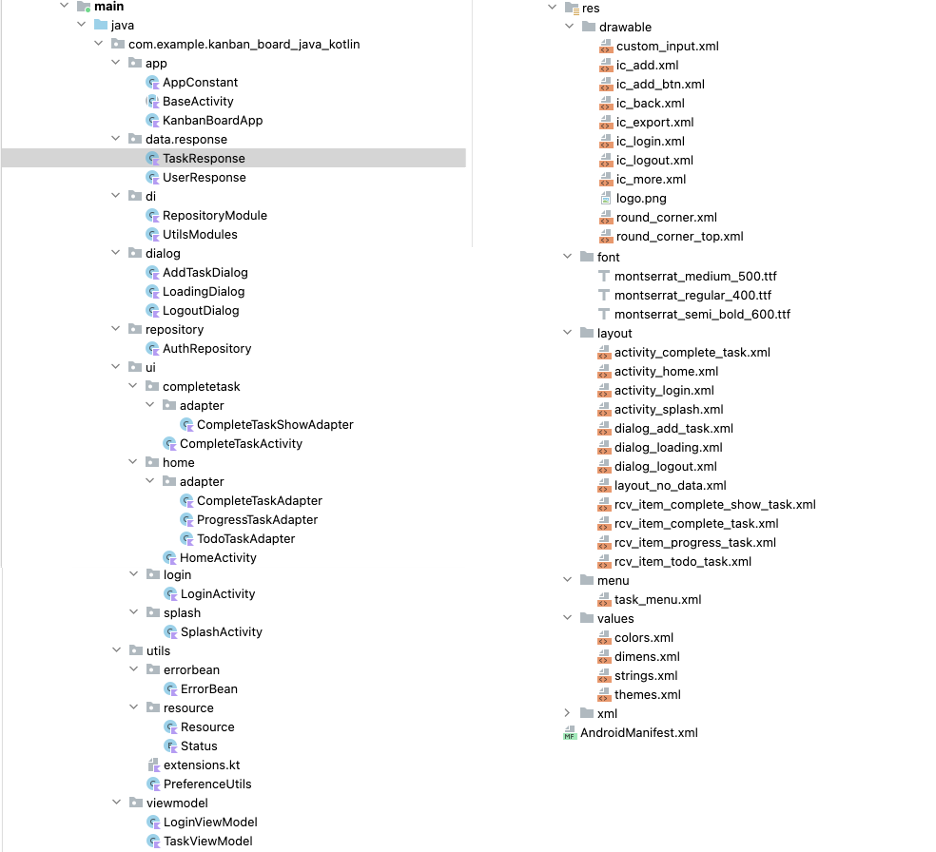
\includegraphics[scale = 0.8]{img/kotlin_project_struct.png}
    \caption{Kotlin version of the application’s project structuring}
    \label{fig:kotlin_project_struct}
\end{figure}
\par
As in Figure \ref*{fig:kotlin_project_struct}, the Kotlin code was orginized into intuitive packages: app for foundational classes like AppConstant and BaseActivity, data.response for handling data models like TaskResponse and UserResponse, and repository for data management, particularly with an AuthRepository to interface with authentication mechanisms. User interfaces were built under the \verb|"ui"| package, divided into sub-packages like \verb|"completetask"|, \verb|"home"|, and \verb|"login"|, each containing activities and adapters for respective functionalities. Utility classes were stored in utils, with error handling and resource management centralized for accessibility.
\par
The resource directory was meticulously structured with drawable resources for UI elements, layout XML files for defining user interfaces, and values for managing themes, strings, and dimensions, ensuring a consistent and visually appealing design. The AndroidManifest.xml was crucial in determining the application's configuration and permissions.
\par
This Kotlin project, despite its inherent challenges, demonstrated the robustness of MVVM in Android development. It enabled a clean separation of business logic from the front end, improving the application's testability and scalability. Our design approach was heavily influenced by the clean architecture principles outlined in Robert C. Martin's works \cite{martin2009clean}, focusing on creating a scalable, maintainable structure that could efficiently accommodate future enhancements and changes.

\subsubsection{Java Application Development}
\begin{figure}[htbp]
    \centering
    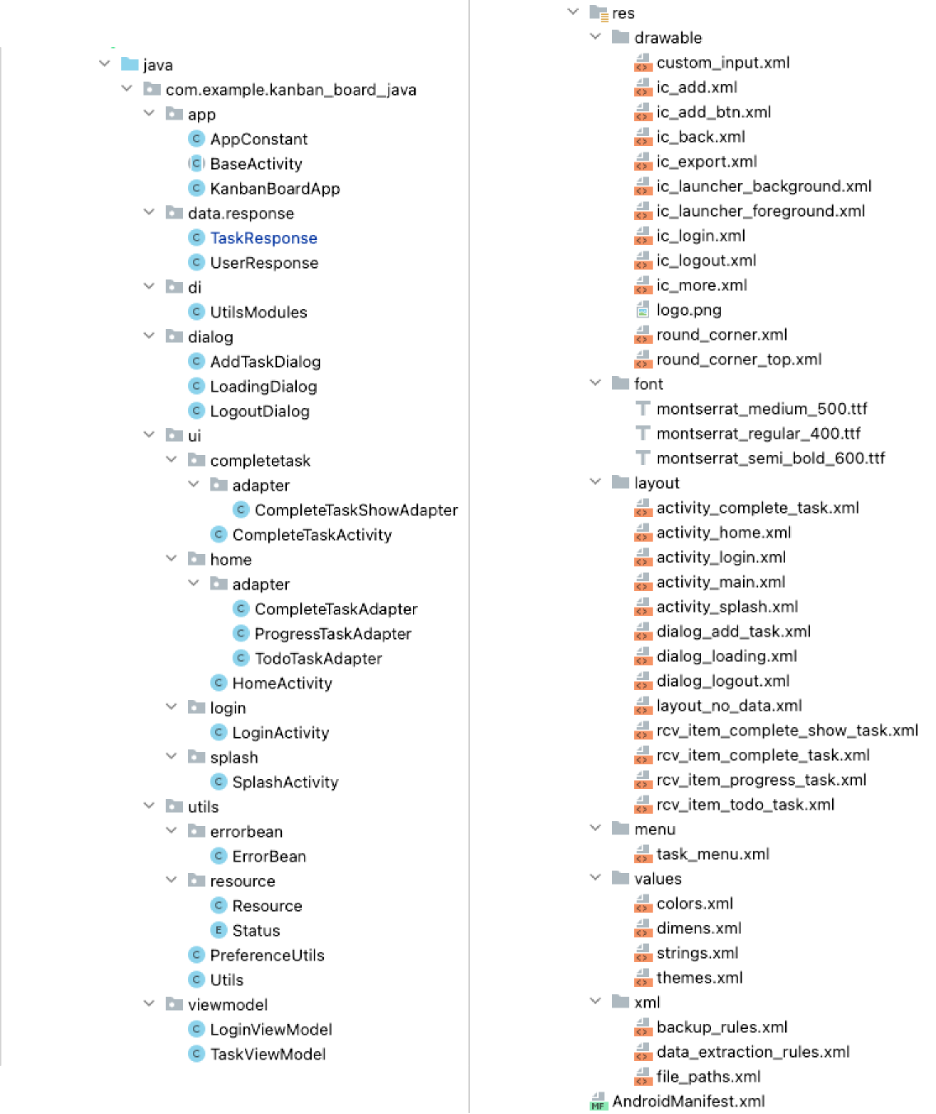
\includegraphics[scale = 0.8]{img/java_project_struct.png}
    \caption{Java version of the application’s project structuring}
    \label{fig:java_project_struct}
\end{figure}
\par
Upon completing the Kotlin project, focus shifted to developing the Android application's Java version. To maintain consistency with the Kotlin version, advanced decompiling tools were implemented to facilitate the conversion of Kotlin code into Java. This approach significantly streamlined the development process, as the tools automatically translated the Kotlin code into Java, maintaining a similar project structure and functionality as outlined in the Kotlin project.
\par
Compile tools proved remarkably effective given the tight project timeline and the need to expedite development without sacrificing code quality. By directly converting the Kotlin code to Java, considerable development time and effort were saved, allowing a focus on refining the Java application and ensuring its robustness and reliability. The entire process of translating and adjusting the Java project took approximately four hours.
\par
The Figure \ref{fig:java_project_struct} indicates that the resultant Java project was structured similarly to the Kotlin version. It included the same packages, such as \verb|"app"| for core application setups such as AppConstant and BaseActivity, \verb|"data.response"| for data models (TaskResponse, UserResponse), and \verb|"repository"| for handling data operations (AuthRepository). The user interface was organized under the \verb|"ui"| package with sub-packages for different functionalities, mirroring the Kotlin setup. Furthermore, utility classes were organized under \verb|"utils,"| and resources were meticulously arranged as in the Kotlin project.
\par
Compression tools ensured consistency between the two projects and enhanced maintainability and scalability, thanks to the established structure and the robustness of the MVVM architecture used in both the Kotlin and Java projects. In conclusion, the strategic use of decompile tools proved essential in meeting our project deadlines efficiently while maintaining high code quality standards and application performance.
\subsection{SonarQube Code Inspection and Open Source Projects}
To commence our discourse, let us delve into a comprehensive comprehension of SonarQube and its purpose. SonarQube is an open-source platform widely utilized for continuous code quality inspection through static analysis. It automatically reviews code to identify bugs, code smells, and security vulnerabilities across various programming languages \cite{hegedHus2022static}. It is a popular tool in academia and industry for managing technical debt, with a significant user base exceeding 120,000 worldwide \cite{lenarduzzi2019technical}. SonarQube tracks and manages technical debt by monitoring issue fixes and code quality improvements over multiple system revisions \cite{tan2021evolution}. Additionally, it calculates various metrics like lines of code and code complexity, ensuring code compliance with specific coding rules for common programming languages \cite{kawuma2022empirical}.
\par
SonarQube's effectiveness extends to cognitive complexity reduction, as it integrates metrics positively correlated with source code understandability, making it a valuable tool for developers \cite{saborido2022automatizing}. The platform allows for detecting violations, known as issues, aiding in predicting changes through coding rule violations \cite{tollin2017change}. Furthermore, SonarQube is instrumental in identifying software metrics and technical debt through static analysis, consolidating the functionalities of tools like Checkstyle and PMD \cite{guamansonarqube}.
\subsubsection{Issue Severity in SonarQube}
Within the scope of our study, considerable emphasis has been placed on the severity levels of issues discovered through SonarQube. These levels play a pivotal role in determining the prioritization of code corrections and comprehending the possible implications on application security and performance. SonarQube classifies each identified issue into one of its five severity levels, offering developers a guiding language to address the most critical problems as a priority.
\begin{itemize}
    \item \textbf{BLOCKER:} Represents bugs with a high probability of impacting the application's behavior in production. Examples include memory leaks or unclosed JDBC connections. These are critical and require immediate attention and resolution.
    \item \textbf{CRITICAL:} Issues that might have a lower probability of impacting the application's production behavior or represent security flaws, such as an empty catch block or SQL injection vulnerabilities. These issues necessitate a prompt review.
    \item \textbf{MAJOR:} Quality flaws that could significantly impact developer productivity, such as uncovered code, duplicated blocks, or unused parameters. While these may not immediately affect application functionality, they impede efficient code management and scalability.
    \item \textbf{MINOR:} Minor quality flaws that may slightly affect developer productivity, like overly long lines or "switch" statements with fewer than three cases. These are less critical but still warrant consideration for code quality improvement.
    \item \textbf{INFO:} Issues that are neither bugs nor quality flaws, but rather findings that may be useful for code optimization or future reference without requiring immediate action.
\end{itemize}


\subsubsection{Setting Up SonarQube Environment}
Measures were taken to ensure robust code quality analysis for the project by setting up a SonarQube environment. The first step involved installing Docker on the local machine, which was necessary to run the SonarQube server. After completing the installation, the SonarQube setup was initiated.
\par
Using the terminal on a Mac, the SonarQube Docker \cite{Docker} image was pulled by executing the command:
\begin{lstlisting}[language=bash]
    $ docker pull sonarqube: 9.9.4.87374-community 
  \end{lstlisting}
  Once completed, it was confirmed that no existing Docker containers were running using the command:
\begin{lstlisting}[language=bash]
    $ docker ps -a 
\end{lstlisting}
before installing new instance. With the command \texttt{docker run -d — name\newline sonarqube -p 9000:9000 sonarqube:9.9.4.87374-community} SonarQube server was started. A subsequent \texttt{docker ps -a} check confirmed that SonarQube was active and running without issues.
\par
To verify the setup, SonarQube was accessed at the local URL http://localhost:9000/ and logged in using the default credentials: Username \texttt{admin} and Password \texttt{admin}. Seeing that SonarQube was correctly set up and operational with this step.
\par
Since SonarQube does not support Dart natively, the programming language used for the Flutter project, a plugin called sonar-flutter \cite{flutter_sonar} was installed, developed by the Flutter community. This plugin allowed Dart code analysis to be integrated into the SonarQube environment, enabling the maintenance of high code quality standards and consistency across development efforts. This integration proved essential for leveraging SonarQube's capabilities to meet the project's needs.
\subsubsection{Applying SonarQube Analysis to the Kanban Board Project}
The integration of SonarQube into the development process of the Kanban board application was instrumental in ensuring high code quality across three different programming languages: Kotlin, Java, and Dart. This section details the steps taken for each language to set up and utilize SonarQube for continuous inspection of code quality.

\textbf{Kotlin-Based Kanban Board Implementation:}
\begin{enumerate}
    \item Setting Up SonarQube: Docker was used to host SonarQube, ensuring a consistent environment. The SonarQube server was accessible at http://localhost:9000 after initiating the Docker container with the command: \texttt{docker run -d — name sonarqube -p 9000:9000 sonarqube: 9.9.4.87374-community}
    \item Project Configuration: In the Kotlin project, the SonarQube Gradle plugin was added to the build.gradle file (apply plugin: \verb|"org.sonarqube"|), and necessary configurations were set within the sonarqube block to specify the project key, name, sources, and exclusions.
    \item Running the Analysis: The analysis was triggered via the command \texttt{./gradlew sonarqube -Dsonar.host.url=http://localhost:9000 \newline-Dsonar.login=\$TOKEN} sending the code metrics to SonarQube and generating a detailed report on code quality.
\end{enumerate}

\textbf{Java-Based Kanban Board Implementation:}
\begin{enumerate}
    \item SonarQube Installation and Configuration: Similar steps were followed in the Kotlin implementation. Docker was used to deploy SonarQube, and the Java project was configured with the SonarQube plugin in the build.gradle file.
    \item Analysis Configuration: Detailed properties were set in the sonarqube block of the build.gradle file, focusing on Java-specific paths and setting appropriate exclusions to filter out generated and test code.
    \item Executing SonarQube Analysis: The SonarQube analysis for the Java project was executed using the same Gradle command. It analyzed the code quality and identified potential issues.
\end{enumerate}
\begin{figure}[htbp]
    \centering
    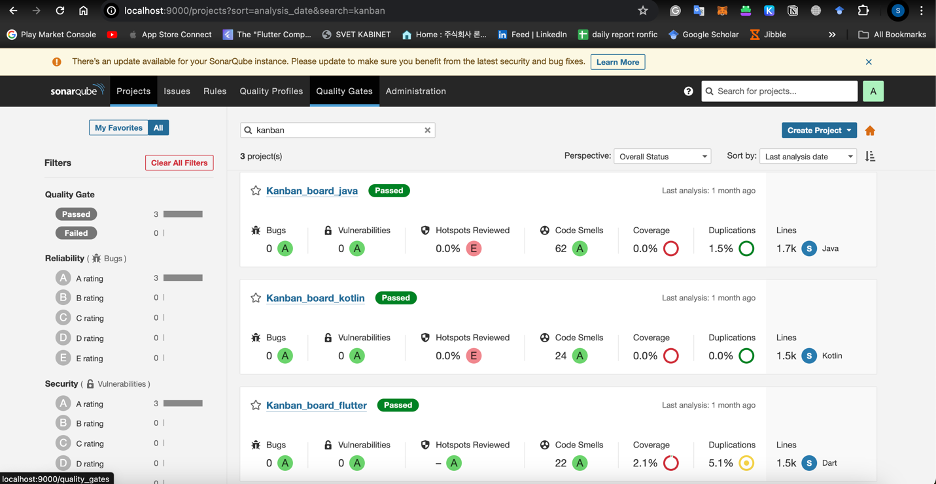
\includegraphics[scale = 0.8]{img/sonarqube_dashboard.png}
    \caption{SonarQube Dashboard Overview: Code Quality Metrics for Kanban Board Projects in Flutter, Kotlin, and Java}
    \label{fig:sonarqube_dashboard}
\end{figure}
\textbf{Flutter-Based Kanban Board Implementation:}
\begin{enumerate}
    \item Plugin Installation for Dart Support: Since SonarQube does not officially support Dart, a third-party plugin (sonar-flutter-plugin-0.4.0.jar) was downloaded and added to the Docker container hosting SonarQube to enable Dart analysis.
    \item Project Configuration for Flutter: In the Flutter project directory, a sonar-project.properties file was created, specifying the project key, name, and SonarQube token. This file also defined the source directories and set exclusions for files that should not be analyzed.
    \item Running SonarQube Analysis: The Flutter project analysis was initiated with the command sonar-scanner after setting the necessary configurations in the properties file and running tests to generate coverage data.
\end{enumerate}

\subsection{Setting Up an Automated Pipeline for SonarQube Analysis of Open Source Projects}

In the initial stages of the project, the inclusion of open-source project analysis was not planned. However, after implementing SonarQube into the Kanban board application, it was realized that deriving a statement based on a single project code written by one developer would not be sufficient to claim that one programming language or framework is better. To address this issue, SonarQube was implemented into GitHub open-source projects. A total of 42 open-source projects were selected from GitHub based on the number of forks and stars. With the Kanban board app developed during this research using three languages, the number of projects for analysis was 15 per language (14 open-source and 1 project developed internally). Tables with 15 projects in 3 languages are included in Appendix \ref{app:a}.
\par
The selected projects were categorized into different types to ensure a diverse and comprehensive analysis. The categories included:
\begin{itemize}
    \item Productivity and Task Management
    \item Finance and Utility Tools
    \item Entertainment and Media
    \item Health and Fitness
    \item Communication and Social Networking
    \item Educational and Development Tools
    \item Security and Privacy
    \item e-commerce
\end{itemize}
This categorization helped in analyzing the projects more effectively based on their specific functionalities and use cases.
\par
However, a significant challenge was encountered due to the lengthy process of implementing SonarQube into the Kanban board application. It was noticed that creating a project on the SonarQube Dashboard and configuring data per language would be too time-consuming. Therefore, the intention was to automate processes such as downloading a GitHub project, creating a project in SonarQube, generating a token for the downloaded project, and saving tokens and other project configurations on the downloaded open-source projects. The first step in the automation process was learning about the APIs provided by SonarQube \cite{sonarQube}. The Python script used for this automation is included in Appendix \ref{app:a2}, along with a detailed explanation.
\par
In brief, the script downloaded open-source projects from GitHub, created a project with the same name on SonarQube, generated a token for that project, and saved all credentials in a text file for Java/Kotlin projects and a .yaml file for Flutter projects. The automation process helped save time, allowing more focus on project structuring rather than performing repetitive tasks.
\par
After finishing the project preparation, each project still needed to be opened and configured. Once the configuration was completed as described earlier, reports were received within SonarQube. Another API provided by SonarQube was used, and another Python script was programmed, which is included in Appendix \ref{app:a3}. This script was one of the final steps of the development, helping to obtain the required statistics for the research.
